\documentclass[10pt,t,svgnames]{beamer}

\usetheme{metropolis} % use metropolis theme

\usepackage{../solarized}         % use solarized themed listings
\usepackage{../stack}             % use the tikzstack environment
\usepackage{appendixnumberbeamer} % do not number appendix frames
\usepackage[scale=3]{ccicons}     % creative commons icons

% fix-up the handling of the notes pages
\ifnotes
  \hypersetup{final}
  \usepackage{pgfpages}
  \setbeamertemplate{note page}[plain]
  \setbeameroption{show notes on second screen=right}
  \AtBeginNote{%
    \let\enumerate\itemize%
    \let\endenumerate\enditemize%
  }
\fi

% overrides default description environment
\newlength\wideleftmargin{}
\newlength\tightleftmargin{}
\newlength\diffleftmargin{}
\setlength\wideleftmargin{6em}    % controls location of term (> is more left)
\setlength\tightleftmargin{1.5em} % controls location of description (same)
\setlength\diffleftmargin{\dimexpr\wideleftmargin-\tightleftmargin}
\makeatletter
\providecommand{\nextline}{
  \setlength\labelwidth{\tightleftmargin}
  \setlength\leftmargin{\tightleftmargin}
  \advance\linewidth\diffleftmargin{}
  \advance\@totalleftmargin-\diffleftmargin{}
  \parshape\@ne\@totalleftmargin\linewidth{}
  \setlength\itemsep{1.5ex}
}
\makeatother
\let\origdescription\description
\let\endorigdescription\enddescription
\renewenvironment{description}{\origdescription\nextline}{\endorigdescription}

%-------------------------------------------------------------------------------

\usepackage{tabularx} % tables

\title{Computer systems}
\date{}
\author{College of Saint Benedict \& Saint John's University}
\begin{document}
  \maketitle

  \begin{frame}[c]{great insights of computer science\footnotemark}
  %{{{1
    \begin{description}
      \item[Bacon, Leibniz, Boole, Turing, Shannon, \& Morse] \hfill \\
        There are only \textbf{two nouns} that a computer has to deal with in
        order to represent ``anything'': 0, 1.
    \end{description}

    \note[item]{``anything'': there are some things computers cannot do --- like
      determine if a program will ever finish.}

    \footnotetext[1]{\href{https://en.wikipedia.org/wiki/Computer\_science\#The\_great\_insights\_of\_computer\_science}{The great insights of computer science}~/~\href{http://creativecommons.org/licenses/by-sa/3.0}{CC~BY-SA~3.0}}
  %}}}1
  \end{frame}

  \begin{frame}[c]{great insights of computer science, cont'd}
  %{{{1
    \begin{description}
      \item[Turing] \hfill \\
        There are only \textbf{five verbs} that a computer has to perform in
        order to do ``anything'':
        \begin{enumerate}
          \item move left one location;
          \item move right one location;
          \item read symbol at current location;
          \item print 0 at current location;
          \item print 1 at current location.
        \end{enumerate}
    \end{description}
  %}}}1
  \end{frame}

  \begin{frame}[c]{great insights of computer science, cont'd}
  %{{{1
    \begin{description}
      \item[Boehm and Jacopini] \hfill \\
        There are only \textbf{three grammar rules} needed to combine these
        verbs (into more complex ones) that are needed in order for a computer
        to do "anything":
        \begin{enumerate}
          \item \emph{sequence}: first do this, then do that;
          \item \emph{selection}: IF such-and-such is the case, THEN do this,
            ELSE do that;
          \item \emph{repetition}: WHILE such-and-such is the case DO this.
        \end{enumerate}
    \end{description}
  %}}}1
  \end{frame}

  \begin{frame}[fragile]{a simple language}
  %{{{1
    \begin{enumerate}
      \item two nouns
      \item five verbs
      \item three grammar rules
    \end{enumerate}
    \vspace{\baselineskip}

    \begin{tabular}{l|l}
      \hline
      \texttt{\textless}    & move left one location\\
      \texttt{\textgreater} & move right one location\\
      \texttt{0}            & print \texttt{0} at current location\\
      \texttt{1}            & print \texttt{1} at current location\\
      \texttt{[}            & if current location is \texttt{0}, then go to
                              instruction after matching \texttt{]}\\
      \texttt{]}            & go to matching \texttt{[} instruction\\
      \hline
    \end{tabular}

    \begin{termblock}
    1>1>0>1>0<<<<[0>]1
    \end{termblock}

    \note[item]{\emph{sequence}: start at left-most instruction and progress a
      single instruction to the right}
    \note[item]{\emph{selection} and \emph{repetition:}
      \texttt{[}\dots\texttt{]} provide both --- repetition is just fancy
      selection}
  %}}}1
  \end{frame}

  \begin{frame}[fragile]{a simple language, cont'd}
  %{{{1
    \vspace{.5\baselineskip}

    \begin{tabular}{l|l}
      \hline
      \texttt{\textless}    & move left one location\\
      \texttt{\textgreater} & move right one location\\
      \texttt{0}            & print \texttt{0} at current location\\
      \texttt{1}            & print \texttt{1} at current location\\
      \texttt{[}            & if current location is \texttt{0}, then go to
                              instruction after matching \texttt{]}\\
      \texttt{]}            & go to matching \texttt{[} instruction\\
      \texttt{\string^}     & add one to the 4-bit number ending at the current
                              location\\
      \hline
    \end{tabular}
    \\[.25\baselineskip]
    \scriptsize{\texttt{\string^} replaces the sequence \texttt{>0<<<<[0>]1}}
    \normalsize

    \begin{termblock}
    1>1>0>1^
    \end{termblock}

    \note[item]{let's add another instruction to increment a number by one}
    \note[item]{we have introduced some \emph{abstraction}}
  %}}}1
  \end{frame}

  \begin{frame}[fragile]{abstraction}
  %{{{1
    \begin{description}
      \item [abstraction] \hfill \\
        A mechanism and practice to reduce and factor out details so that one
        can focus on a few concepts at a time. \\[.5\baselineskip]
        \emph{Abstraction allows program designers to separate categories and
        concepts related to computing problems from specific instances of
        implementation.}\footnote{\href{https://en.wikipedia.org/wiki/Abstraction\#In\_computer\_science}{Abstraction}~/~\href{http://creativecommons.org/licenses/by-sa/3.0}{CC~BY-SA~3.0}}
    \end{description}
  %}}}1
  \end{frame}

  \begin{frame}[fragile]{types of abstraction}
  %{{{1
    \begin{description}
      \item [data abstraction] \hfill \\
        The separation of a data type’s logical properties from its concrete
        implementation. \\[.5\baselineskip]
        In fact, a data type is a data abstraction.
        \begin{termblock}
    boolean found := false
        \end{termblock}
      \item [control abstraction] \hfill \\
        The separation of the behavior of a set of actions from its concrete
        implementation. \\[.5\baselineskip]
        One of the main purposes of programming languages. \\[.5\baselineskip]
        \begin{termblock}
    a := (2 + 3) / 4
        \end{termblock}
    \end{description}

    \note{
      \begin{itemize}
        \item Data abstraction --- take 8 bits, how do you know how to interpret
          the 8 bits? You will need to know if it is an: integer, a
          floating-point value, or something else\dots all three are
          abstractions of the bits
        \item Here is an example --- How is an 32-bit number actually stored in
          our machine? $0x0000010F=271$
      \end{itemize}
      \begin{itemize}
        \item In the example code, \texttt{:=}, \texttt{+}, and \texttt{/} are
          all examples of control abstraction
        \item What vale does \texttt{a} hold?
          \begin{itemize}
            \item You will need to now what data abstraction we are using for
              the numbers \texttt{2}, \texttt{3}, and \texttt{4}, so that you
              know their logical properties, like how addition and division of
              two of them works
          \end{itemize}
        \item Other examples include decisions, iterations, functions
      \end{itemize}
      \begin{itemize}
        \item Where do classes in Java fit?
      \end{itemize}
    }
  %}}}1
  \end{frame}

  \begin{frame}{abstraction levels}
  %{{{1
    \vspace{3ex}
    \begin{columns}
      \begin{column}{.34\textwidth}
        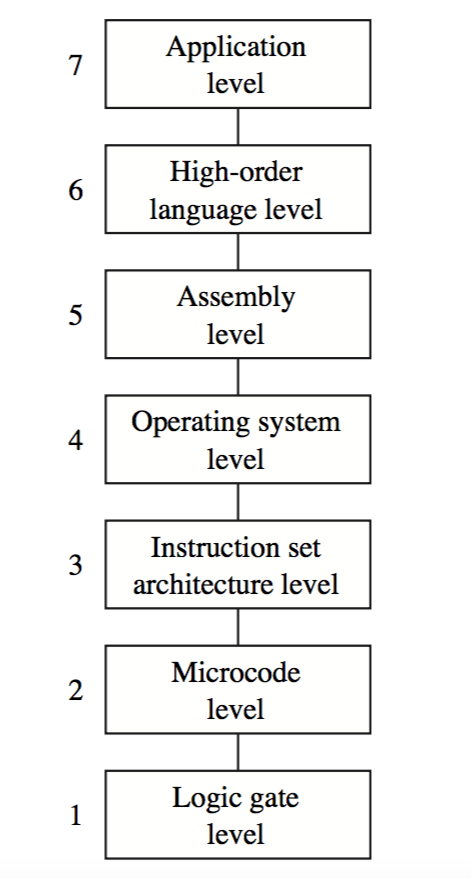
\includegraphics[width=\textwidth]{levels.png}\\
        \hfill \tiny{\href{http://computersystemsbook.com/resources}{Figure P.1}}
      \end{column}
    \end{columns}
  %}}}1
  \end{frame}

  \begin{frame}{history of abstraction}
  %{{{1
    \vspace{3ex}
    \begin{columns}
      \begin{column}{.82\textwidth}
        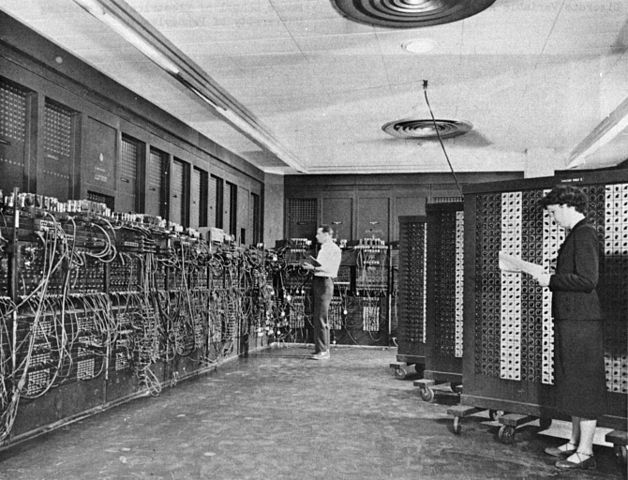
\includegraphics[width=\textwidth]{Eniac.jpg}\\
        \hfill
        \tiny{\href{https://commons.wikimedia.org/w/index.php?curid=55124}{U.S.~Army~Photo}~/~Public~Domain}
      \end{column}
    \end{columns}

    \note[item]{Circa 1946 --- World War II}
    \note[item]{LG1 \& ISA3}
    \note[item]{Six women: Kay McNulty, Marlyn Wescoff, Ruth Lichterman, Betty
      Jean Jennings, and Fran Bilas, programmed the first large-scale general
      purpose machine, ENIAC, to compute ballistics trajectories. Programming
      was done by reorganizing wiring of plugboards.}
  %}}}1
  \end{frame}

  \begin{frame}{history of abstraction, cont'd}
  %{{{1
    \vspace{3ex}
    \begin{columns}
      \begin{column}{.82\textwidth}
        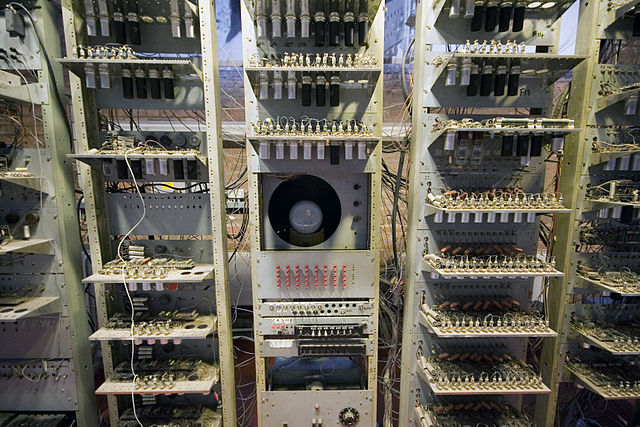
\includegraphics[width=\textwidth]{SSEM.jpg}\\
        \hfill
        \tiny{\href{https://commons.wikimedia.org/w/index.php?curid=55124}{SSEM
        Manchester museum close up}~/~\href{http://creativecommons.org/licenses/by-sa/3.0}{CC~BY~3.0}}
      \end{column}
    \end{columns}

    \note[item]{Circa 1948}
    \note[item]{LG1 \& ISA3}
    \note[item]{Stored program in memory. Programs were entered in binary form
      by stepping through each word of memory in turn, and using a set of 32
      switches known as the input device to set the value of each bit of each
      word to either 0 or 1.}
  %}}}1
  \end{frame}

  \begin{frame}{history of abstraction, cont'd}
  %{{{1
    \vspace{3ex}
    \begin{columns}
      \begin{column}{.52\textwidth}
        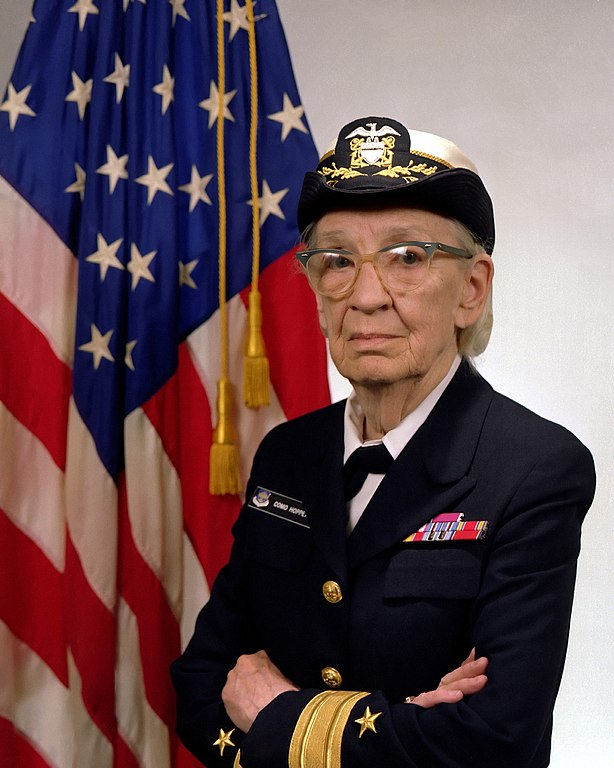
\includegraphics[width=\textwidth]{Grace_Hopper.jpg}\\
        \hfill
        \tiny{\href{https://en.wikipedia.org/wiki/File:Commodore\_Grace\_M.\_Hopper,\_USN\_(covered).jpg}{Commodore~Grace~M.~Hopper,~USN}~/~Public~Domain}
      \end{column}
    \end{columns}


    \note{
      \begin{itemize}
        \item Circa 1951
        \item ASM5 \& HOL6
        \item assembly and high-order languages were developed around the same
          time
        \item Assembly programs are machine-specific, 1-to-1 mapping between
          assembly instructions and machine instructions
        \item some early programming languages still in use today:
          \begin{itemize}
            \item FORTRAN (1954)
            \item LISP (1958)
            \item COBOL (1959)
            \item ALGOL (1958)
          \end{itemize}
      \end{itemize}
    }
  %}}}1
  \end{frame}

  \begin{frame}{history of abstraction, cont'd}
  %{{{1
    %\vspace{3ex}
    %\begin{columns}
    %  \begin{column}{.52\textwidth}
    %    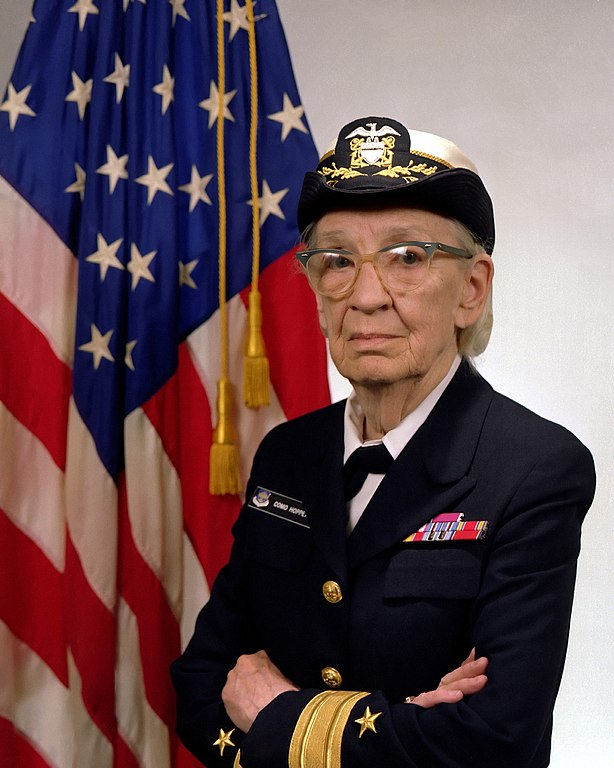
\includegraphics[width=\textwidth]{Grace_Hopper.jpg}\\
    %    \hfill
    %    \tiny{\href{https://en.wikipedia.org/wiki/File:Commodore\_Grace\_M.\_Hopper,\_USN\_(covered).jpg}{Commodore~Grace~M.~Hopper,~USN}~/~Public~Domain}
    %  \end{column}
    %\end{columns}

    \note{
      \begin{itemize}
        \item Circa 1956
        \item OS4
        \item operating system is a piece of software that runs other pieces of
          software
        \item allow multi-tasking and multi-user environments
        \item gives software an interface to hardware --- it manages hardware
          resources
      \end{itemize}
    }
  %}}}1
  \end{frame}

  \begin{frame}{hardware abstraction}
  %{{{1
    \vspace{3ex}
    \begin{columns}
      \begin{column}{\textwidth}
        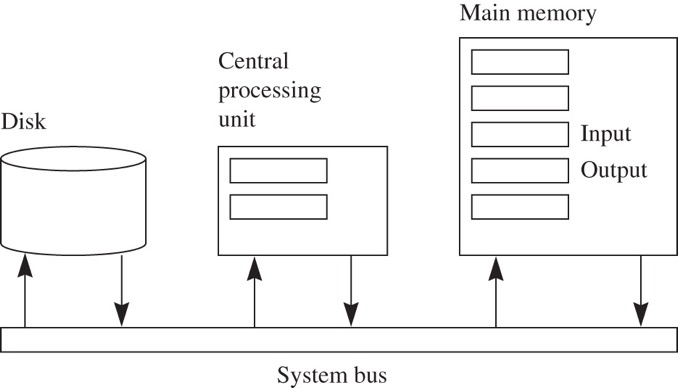
\includegraphics[width=\textwidth]{system.jpg}\\
        \hfill
        \hfill \tiny{\href{http://computersystemsbook.com/resources}{Figure 1.9}}
      \end{column}
    \end{columns}

    \note{
      \begin{itemize}
        \item Ask students what the different parts of the picture are
      \end{itemize}
      \begin{itemize}
        \item The only instructions that a CPU can perform are hard-wired into
          its circuits (LG1) --- example: \texttt{add} is hard-wired,
          \texttt{multiply} is written in MC2
        \item MC2 requires an interpreter to be hard-wired into CPU to translate
          MC2 to LG1
        \item CPU can only compute on values in \emph{registers} --- modern
          machine has on the order of tens of registers
      \end{itemize}
      \begin{itemize}
        \item Show demonstration with SimHYMN
      \end{itemize}
      \begin{itemize}
        \item \emph{memory-mapped i/o} --- the input and output devices are
          treated as special locations in a process' address space --- this is
          handled by the OS
      \end{itemize}
    }
  %}}}1
  \end{frame}

  \begin{frame}{hardware abstraction, cont'd}
  %{{{1
    \begin{tikzpicture}[
      scale=.3,
      auto,
      block/.style={
        rectangle,
        draw,
        fill=blue!20,
        text width=6em,
        rounded corners,
      },
      line/.style={
        draw,
        -latex'
      }
    ]
      % Place nodes
      \node [block, label=left:HOL] (hol6) {j := i * 5};
      \node [block, below of=hol6, label=left:ISA, node distance=2cm] (isa3) {load i\\mult 5\\store j};
      \node [block, right of=isa3, node distance=6cm,label=right:MC] (mc2) {load
        i\\store reg1\\load 0\\store reg2\\load 5\\store reg3\\loop:\\~~~load
        reg2\\~~~add reg1\\~~~store reg2\\~~~load reg3\\~~~sub 1\\~~~store
        reg3\\~~~jpos loop\\load reg2\\store j};
      \node [block, below of=isa3, node distance=2.5cm, font=\ttfamily,label=left:LG] (lg1) {--|``-.\\
~~~~|~~~~~~:--\\
--|..-`};
      % Draw edges
      \path [line] (hol6) -- node {compiler} (isa3);
      \path [line] (isa3) -- node[text width=6em] {hardware interpreter} (mc2);
      \path [line] (mc2) -- node[text width=6em] {hardware decoder} (lg1);
    \end{tikzpicture}

    \note[item]{With the introduction of MC, there is not a 1-to-1 mapping
      between IS3 and capabilities of CPU}
    \note[item]{Now, ISA defines capabilities and MC implements them if LG
      doesn't}
  %}}}1
  \end{frame}

  \begin{frame}{software abstraction}
  %{{{1
    \begin{description}
      \item [algorithm] \hfill \\
        a set of \emph{instructions} that, when carried out in the proper
        sequence, solves a problem in a finite amount of time
      \item [program] \hfill \\
        an algorithm written in a language that is understandable by a computer,
        i.e., that can be executed on a computer
    \end{description}
    \note{
      \begin{itemize}
        \item what is an instruction
          \begin{itemize}
            \item this is where people get hung up, \emph{instruction} is not
              necessarily an instruction that a machine can understand
            \item but, if the algorithm is for a computer, the instruction
              should be something that the computer is capable of
          \end{itemize}
      \end{itemize}
    }
  %}}}1
  \end{frame}

  \begin{frame}[fragile]{algorithms}
  %{{{1
    \begin{termblock}
    while i is greater than or equal to 0
      print i
      subtract 1 from i
    \end{termblock}
    \vspace{2\baselineskip}
    \begin{termblock}
    print the numbers from i to 0
    \end{termblock}

    \note[item]{I consider both of these algorithms}
  %}}}1
  \end{frame}

  \begin{frame}{system performance}
  %{{{1
    $$\frac{\textrm{time}}{\textrm{program}}=\frac{\textrm{instructions}}{\textrm{program}}\times\frac{\textrm{cycles}}{\textrm{instruction}}\times\frac{\textrm{time}}{\textrm{cycle}}$$\\[2\baselineskip]

    \begin{block}<2>{try it yourself}
      Suppose your CPU is rated at 2.5 GHz and you execute a program task on
      your app that requires the execution of 16 million ISA3 instructions. If
      each ISA3 instruction executes an average of 3.7 MC2 instructions, what is
      the execution time of the program task in seconds?
    \end{block}

    \note{
      \begin{itemize}
        \item Note the prefix indicate powers of 10
      \end{itemize}
      \begin{itemize}
        \item $\frac{\textrm{instructions}}{\textrm{program}}$ is \# of ISA 3
          instructions in the program
        \item $\frac{\textrm{cycles}}{\textrm{instruction}}$ is average \# of
          MC2 instructions per ISA3 instruction
        \item $\frac{\textrm{time}}{\textrm{cycle}}$ is $\frac{1}{\textrm{CPU
          frequency}}$ -- also called the \emph{period}
      \end{itemize}
    }
    \note<2>{
      \begin{itemize}
        \item
          $(16\times10^6)\times(3.7)\times(1/(2.5\times10^9))=23.7\mathrm{ms}=23.7\times10^{-3}\approx0.024\mathrm{s}$
      \end{itemize}
    }
  %}}}1
  \end{frame}

  \begin{frame}{bandwidth}
  %{{{1
    $$\textrm{information}=\frac{\textrm{information}}{\textrm{time}}\times\textrm{time}$$\\[2\baselineskip]

    \begin{block}<2>{try it yourself}
      One of the largest (but not the largest, but very close to it),
      telecommunications companies in the U.S., offers an internet product
      called Continuum that promises up to 100 Mb/s for the low price of
      \$45/month. A smaller and slightly less popular telecomm company offers a
      competing product offering up to 25 Mb/s for \$30/month. If I have two
      devices capable of streaming Netflix HD, which product should I choose?
      Construct an argument to explain to the customer service representative
      for the company whose product you do not choose, why.
    \end{block}

    \note<2>{
      \begin{itemize}
        \item Netflix HD transfers about 3 GB/hour
        \item $3\textrm{GB/hour}=3*1000*1000*1000*8=24,000,000,000 \textrm{b/hour}=24,000 \textrm{Mb/hour}\approx6.6 \textrm{Mb/s}$
      \end{itemize}
    }
  %}}}1
  \end{frame}

  \appendix

  \begin{frame}[c]
  %{{{1
    \begin{center}\ccbysa\end{center}

    except where otherwise noted, this worked is licensed under
    \href{http://creativecommons.org/licenses/by-sa/4.0/}{creative commons
    attribution-sharealike 4.0 international license}
  %}}}1
  \end{frame}
\end{document}
